\section{Diseño}
En esta sección se describirá el punto de partida del asistente JiraGPT Next y el diseño que se ha propuesto como mejora para la precisión de las consultas generadas. Se presentarán 3 alternativas utilizando arquitecturas RAG, que buscan dotar al modelo de información sobre la generación de consultas JQL.

Para estas tres propuestas, se ha hecho un estudio del estado del arte y se han consultado varios artículos que tratan de realizar mejoras similares a las expuestas en este trabajo, logrando inspiración en ellos. Por lo que, se van a probar 3 bases de conocimiento distintas con las que aumentar el contexto que posee el modelo y buscar una mejora en la precisión de las respuestas. Se va a utilizar una ontología para representar las reglas del lenguaje de consulta JQL, una base de datos vectorial con embeddings de la documentación de JQL y un Knowledge Graph que contenga los datos de un proyecto real de LKS Next-GobTech. La figura \ref{fig:diagrama_general} muestra un diagrama general de las 3 propuestas.

\begin{figure}[H]
    \centering
    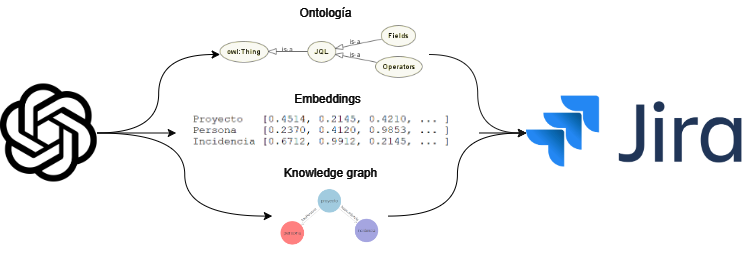
\includegraphics[width=0.95\textwidth]{images/diagrama_general.png}
    \caption{Diagrama de las tres propuestas, simbolizando las 3 bases de conocimiento distintas que van a ser estudiadas.}\label{fig:diagrama_general}
\end{figure}

\subsection{Estado inicial}
La aplicación desarrollada por Joel García y la presentada en este trabajo difieren en la manera de interactuar con el modelo. La aproximación que tomó Joel García fue la de realizar una ejecución de tres fases distintas, interactuando varias veces con el modelo. En el diagrama de la figura \ref{fig:diagrama_joel}, obtenido del trabajo de Joel García~\cite{jiragpt}, muestra el flujo de trabajo de la aplicación JiraGPT Next en su estado inicial.

\begin{figure}[H]
    \centering
    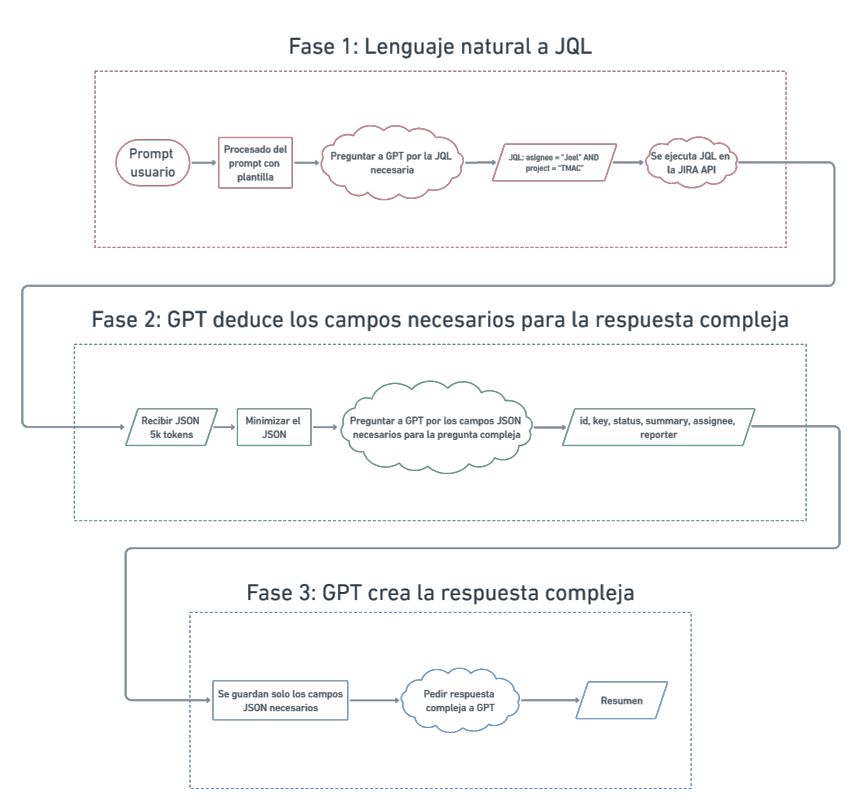
\includegraphics[width=0.95\textwidth]{images/diagrama_joel.png}
    \caption{Diagrama de las tres fases de la aplicación JiraGPT Next en su estado inicial~\cite{jiragpt}.}\label{fig:diagrama_joel}
\end{figure}

Durante la primera fase se preprocesaba la pregunta para adaptarla con plantillas y otorgar algo de contexto e indicaciones al modelo, se enviaba la pregunta y se postprocesaba la respuesta para limpiar cualquier tipo de comentario adicional que imposibilitase la ejecución de la consulta JQL. Durante esta misma fase se realizaba la llamada a la API de Jira con la consulta JQL generada ya procesada y se recogía el JSON devuelto.

La segunda fase consistía en limpiar el JSON para reducir campos de la respuesta que no contienen información relevante. En caso de no haber activado el botón de pregunta compleja, el resultado sería el JSON limpio, que se expone en la interfaz al usuario. En caso de haber activado la pregunta compleja, se haría una segunda llamada al modelo para que decidiese cuáles de los campos del JSON que se han conservado son relevantes para responder a la pregunta.

La tercera fase, que se ejecutaba independientemente de si la pregunta compleja ha sido activada, consistía en una tercera llamada para que realizase un resumen de lo preguntado. De esta manera, el usuario recibía tanto los campos que había solicitado como un resumen que respondiese a su pregunta de manera más directa.

Este proceso utilizaba la libería de Python que ofrece OpenAI para comunicarse con el modelo, de manera que resulta necesario adaptar el código para que funcione con esta librería. Lo que se propone desde este trabajo, también es una mejora en la interacción con el modelo, ya que se va a utilizar Langchain, una librería que permite la abstracción del uso del modelo, por lo que es más sencillo realizar llamadas a cualquier modelo de nuestra elección, sin tener que depender de las librerías de cada uno de los proveedores de estos modelos.

\subsubsection{Precisión inicial}
Para evaluar el estado inicial del modelo se ha de poner en contexto la técnica utilizada para evaluar la precisión: un \textit{benchmark} de 70 preguntas en el que se relaciona cada una con las incidencias que deberían ser recuperadas por el modelo.

La manera en la que se evalúa es ejecutando el conjunto entero de preguntas y comprobando si el asistente ha recuperado exactamente las incidencias contenidas en el conjunto de datos. Esto se decidió de esta manera ya que puede darse el caso en el que diferentes consultas devuelvan las mismas incidencias, lo que se consideraría correcto, con tal de que esas incidencias respondan a la pregunta del usuario.

En el momento de inicio de este trabajo, el asistente JiraGPT Next oscilaba entre un 45 y un 50\% de precisión en la recuperación de incidencias. Este resultado es fruto de una investigación sobre \textit{prompt engineering} realizada previamente por Joel García~\cite{jiragpt}. El objetivo, entonces, es buscar nuevas maneras de mejorar la precisión ofrecida por el modelo.
\subsection{Propuestas}
Se propone utilizar arquitecturas \aclink{RAG} para mejorar la precisión, ofreciendo al modelo información sobre la generación de consultas \aclink{JQL}. La idea detrás de esto es que, al tener un modelo de recuperación que pueda acceder a una base de conocimiento, el modelo de generación pueda generar respuestas más precisas y acordes al contexto proporcionado. Además, se propone un nuevo conjunto de datos:

Si bien el conjunto de datos inicial era robusto, se ha propuesto un nuevo conjunto, de 100 preguntas, que busca, no solo tener más datos, sino hacerlos más diversos y cambiar en cierto modo las preguntas para cubrir el máximo número de casos posible. Este conjunto de datos se ha pensado durante el desarrollo y las diferentes pruebas lanzadas y también se ha usado como apoyo un dataset existente en \textit{Hugging Face}~\cite{datasetHF}.

A continuación, se describirán las distintas alternativas propuestas para mejorar la precisión del modelo JiraGPT Next.

\subsubsection{Ontología}
Durante el inicio de este trabajo se consultaron artículos como \textit{Sequeda et al.}~\cite{sequeda2023benchmark}, que exploraban la posibilidad de utilizar ontologías en el prompt para mejorar la interpretación de los datos y la generación de consultas SQL, logrando resultados prometedores. Partiendo de esta idea, se propone entonces crear una ontología que represente las reglas que existen en las consultas JQL. La información que se pretende representar en la ontología se ha extraído directamente de la documentación oficial de Jira, brindada por Atlassian, donde se detallan las reglas que se deben seguir para la creación de consultas JQL \cite{jiradocs}. Esta ontología serviría para interpretar las reglas que hay que seguir al generar consultas JQL, además, consta de ejemplos en cada una de las clases definidas, que ayuda a comprender mejor el funcionamiento de las reglas.

Para crear esta ontología se ha utilizado el software \textit{Protégé}~\cite{protege}, una herramienta de código abierto para la creación de ontologías desarrollada por la Universidad de Stanford. La ontología se ha desarrollado siguiendo el estándar \textit{Web Ontology Language} (OWL), que es un lenguaje de marcado semántico para publicar y compartir ontologías en la web. OWL es desarrollado por el \textit{World Wide Web Consortium} (W3C) y es una extensión de \textit{Resource Description Framework} (RDF).

Durante esta parte, se considera una ejecución del benchmark como \textit{baseline} para comparar los resultados obtenidos con la ontología y sin ella. Esta primera ejecución se realizaría inyectando el archivo entero de la ontología en el prompt, de manera que el modelo pueda acceder a la información de la ontología y utilizarla para generar consultas más precisas.

Esta aproximación podría presentar resultados que, a priori, parecieran prometedores. Sin embargo, de cara al coste de inyectar un prompt tan grande, no es viable en un entorno de producción. Por ello, se propone una recuperación de información de la ontología dado un campo relevante para la pregunta del usuario. El diagrama en la siguiente figura muestra cómo será la interacción entre el modelo y la ontología.
\begin{figure}[H]
    \centering
    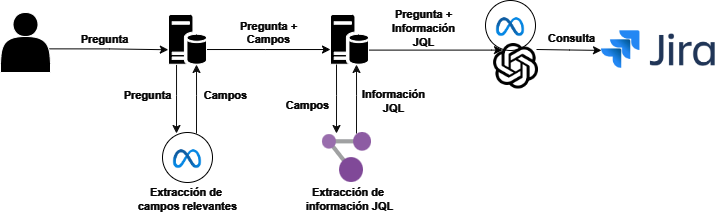
\includegraphics[width=0.95\textwidth]{images/rag_ontologia.png}
    \caption{Diagrama de RAG con ontología}\label{fig:ontologia}
\end{figure}
Si bien una ontología es una manera de representar un espacio de conocimiento, la documentación de Jira no presenta una estructura demasiado compleja que representar con la semántica de una ontología. Podría considerarse que, por ende, no es realmente necesario el uso de una ontología para representar las reglas de JQL. Sin embargo, tras lo realizado en este trabajo, no sería complicado utilizar otra ontología que reuniese información más compleja y permitiese explotar la semántica de la ontología para mejorar la generación de consultas JQL.

\subsubsection{Embeddings}
De igual manera que en el diseño de la ontología, se propone capturar en esta base de datos vectorial la documentación oficial de Jira. Esta base de conocimiento prueba a guardar los embeddings de los diferentes descripciones dentro de la documentación. La información que se ha considerado relevante ha sido cada campo/operador/función y sus respectivos ejemplos. De esta manera, dada una pregunta se podrían obtener los embeddings de las palabras y compararlas con los embeddings de la base de datos, de manera que el modelo obtenga ejemplos de campos relevantes para la pregunta del usuario.

Para capturar toda la información de la documentación se ha diseñado un programa en Python que realiza técnicas de \textit{web scraping} y recorre las entradas de la documentación extrayendo de las tablas los ejemplos. Una vez hecho esto, se guarda en un archivo de texto que será dividido en diferentes partes para ser procesado por el modelo de embeddings.